\chapter{Análisis} \label{chap:analisis}

Dentro de este capítulo, se abordan diversos aspectos clave relacionados con la fase de análisis del proyecto. El enfoque principal es el análisis detallado de los usuarios objetivo \ref{sec:usuariosobjetivos}, donde se exploran sus necesidades, expectativas y limitaciones. Este análisis es esencial para comprender en profundidad el contexto y los requerimientos del sistema.

Además, se presentan los modelos de caso de uso \ref{sec:casodeuso}, que describen las interacciones de los usuarios con el sistema y ayudan a identificar las funcionalidades clave que debe incorporar la solución. 

Se incluyen igualmente los modelos de comportamiento y el modelado de entidades y relaciones \ref{sec:er}. Estos componentes son cruciales para entender la dinámica del sistema y la estructura de datos que soportará.

Al final de este capítulo, se habrá ofrecido una visión estructurada de la solución propuesta, sentando las bases para la obtención de los requisitos necesarios y facilitando el proceso de diseño.

\section{Análisis de Usuarios Objetivo} \label{sec:usuariosobjetivos}

El enfoque de la plataforma web está dirigido principalmente a niños entre los 8 y 18 años, siguiendo la metodología de CODELEARN S.L.. Donde la mayoría de los clientes son estudiantes con poco o ningún conocimiento previo de programación. Es por ello que la plataforma está diseñada para ser intuitiva y flexible, en línea con las recomendaciones de Large y Beheshti sobre el diseño de interfaces para niños \cite{large2005}.

Si tenemos en cuenta la brevedad del período de atención de los niños y su desarrollo cognitivo en curso, se deberán evitar tareas extensas o excesivamente complicadas. Las expectativas y necesidades son diversas, pero comúnmente incluyen una interfaz visualmente atractiva, instrucciones claras y una retroalimentación inmediata tal como especifican Duglas Frye y Elliot Soloway \cite{interfacedesign}. Asimismo, se deben incorporar elementos de gamificación dentro la plataforma con tal mantener el interés y la motivación de los usuarios. 

Finalmente, la plataforma debe ser accesible; es decir, se podrá acceder desde múltiples dispositivos como ordenadores, tablets y smartphones debido a su diseño \textit{Web Responsive}.

\section{Análisis de Requisitos Educativos}

La enseñanza de habilidades de programación dentro de las escuelas está cobrando una gran relevancia \cite{teachingcodingchildren}. Sin embargo, hay una falta de herramientas y enfoques efectivos mucho más allá de herramientas como Scratch \cite{teachingcodingchildren}. Conscientes de esta brecha, se adopta un enfoque fundamentado en evidencia y prácticas académicas sólidas. 

Aunque lenguajes como Scratch y Logo son de los más populares para la educación de niños, se opta por Python, C++, Java y HTML+CSS+JS. Python es conocido por su simplicidad y legibilidad, lo que facilita el aprendizaje para los principiantes \cite{pears2007}. Además, permite una transición fluida a lenguajes más complejos. C++, Java y HTML+CSS+JS, aunque sujetos a debate sobre su idoneidad para principiantes, son cruciales en la industria y la educación. Siendo su relevancia práctica la justificación de su presencia \cite{dewarschonberg}.

Al ir más allá de los enfoques basados en bloques como Scratch, se busca que los niños aprendan la programación basada en texto, más cercana a la realidad. Los ejercicios se organizan por competencias específicas, permitiendo un aprendizaje adaptable y progresivo. Alineando el enfoque con los resultados de investigaciones sobre el tema \cite{document2010}. 

Es importante destacar que el sistema debe ser inclusivo, adaptando los ejercicios al progreso individual del estudiante y con un buen sistema de asistencia. De esta manera, se siguen las directrices recomendadas por Luxton-Reily y Wünsche sobre las características de un buen sistema inteligente para la enseñanza de programación \cite{intelligentturoingprogrammingeducation}, consiguiendo un buen enfoque educativo.

\section{Modelos de Caso de Uso y Escenarios de Uso} \label{sec:casodeuso}

Dentro de esta sección se va a hablar de las interacciones usuario-sistema. En primer lugar, se abordará los modelos de caso de uso \ref{fig:caso_uso}. Debido a que nos proporcionan una visión panorámica, resaltando las posibles interacciones y los actores implicados. Es decir, ayudará a definir lo que el sistema puede hacer y lo que se espera que haga. Además, también se va a especificar los diferentes escenarios de uso, ya que proporcionarán una mejor comprensión de las interacciones específicas pudiendo observar las verdaderas dinámicas del sistema en acción.

Con esta combinación, se establecen las funcionalidades esperadas del sistema y cómo este responderá ante diferentes situaciones y acciones del usuario. Es importante destacar que todos los diagramas que se ven durante la memoria se han realizado mediante PlantULM \cite{planttext}. 

\subsection{Actores del Sistema}

La interacción con la plataforma se basa en tres tipos de usuarios; estudiantes, profesores y administradores. El acceso a la plataforma está restringido a los usuarios registrados, ya que se busca asegurar que cada interacción dentro del sistema se realice en un entorno seguro y personalizado. De esta manera, el sistema es capaz de ofrecer una experiencia adaptada al estudiante y a su progreso.

Los actores identificados en el sistema son:

\begin{itemize}
    \item \textbf{Estudiantes}: Constituyen el grupo principal de usuarios. Su interacción con la plataforma está enfocada en el aprendizaje de programación mediante los recursos educativos disponibles. Los estudiantes tienen acceso a ejercicios, material didáctico, retroalimentación personalizada y un apartado personal para la resolución de dudas.
    \item \textbf{Profesores}: Actúan como facilitadores del proceso de aprendizaje y brindan apoyo emocional a los estudiantes. Entre sus responsabilidades específicas está la corrección de ejercicios de HTML, que requieren una atención más detallada, así como la resolución de dudas y el seguimiento personalizado de estudiantes, especialmente a aquellos que presentan dificultades o inactividad, para motivarles y guiarles en su proceso educativo.
    \item \textbf{Administradores}: Son los usuarios con el mayor nivel de control dentro del sistema. Se encargan de la gestión integral del contenido didáctico y de la administración de los profesores. Su rol es esencial para el mantenimiento y la actualización constante de la plataforma.
\end{itemize}


El diagrama de caso de uso \ref{fig:caso_uso} que se muestra a continuación  ilustra cómo estos actores interactúan con el sistema. Cada actor está asociado con unas acciones específicas y flujos de trabajo dentro de la plataforma, reflejando el enfoque personalizado y la adaptabilidad del sistema.

\begin{figure}[H]
    \centering
    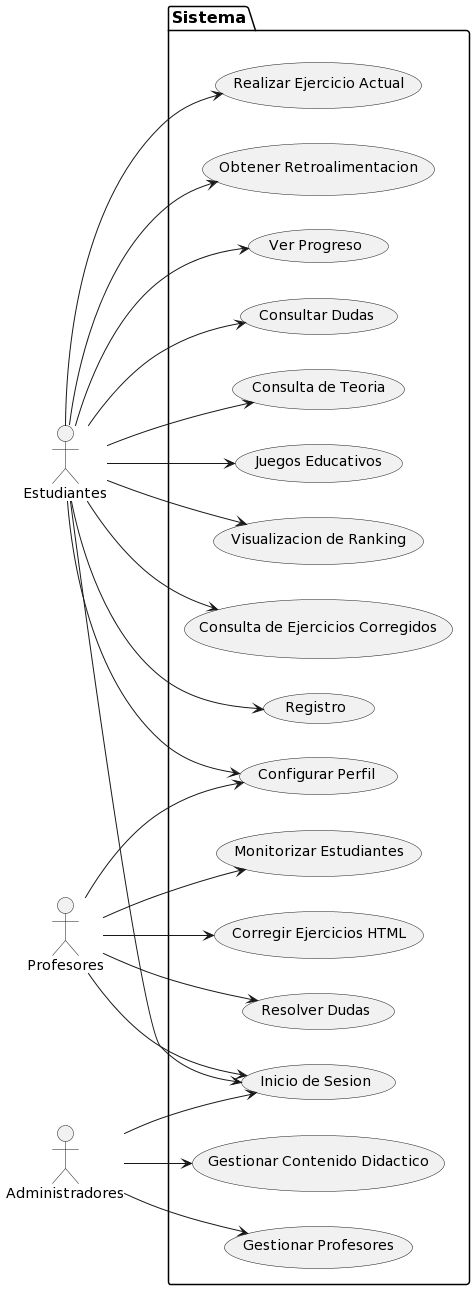
\includegraphics[width=0.4\textwidth]{imagenes/modelo.png}
    \caption{Diagrama de Caso de Uso del sistema}
    \label{fig:caso_uso}
\end{figure}

\subsection{Escenarios de Uso Detallados} \label{sec:comportamiento}

En esta subsección, se realiza un análisis de los escenarios de uso que involucran a los diferentes tipos de usuarios de la plataforma. Para cada escenario, se presentarán tablas detalladas que ofrecen una comprensión clara de cómo los usuarios interactúan con el sistema. Estos escenarios son esenciales para entender las funcionalidades y la respuesta del sistema ante las necesidades de los usuarios.

Los elementos que compondrán cada tabla de escenarios de uso son los siguientes, siguiendo las pautas recomendadas por expertos en usabilidad:

\begin{itemize}
    \item \textbf{ID}: Código de identificación único para cada escenario de uso.
    \item \textbf{Nombre}: Título descriptivo para el escenario de uso.
    \item \textbf{Actor}: Definición de los usuarios implicados en la acción.
    \item \textbf{Descripción}: Breve explicación del escenario de uso. 
    \item \textbf{Precondiciones}: Condiciones previas necesarias para que se inicie el escenario
    \item \textbf{Postcondición}: Estado o resultado alcanzado tras completar el escenario.
    \item \textbf{Flujo}:Detalle de todos los pasos del escenario, incluyendo flujos básicos y alternativos.
\end{itemize}

Los escenarios se centran en aspectos cruciales de la plataforma, enfatizando aquellos factores más relevantes y únicos. Se ha decidido omitir escenarios de uso comunes y autoexplicativos, como el inicio de sesión, registro o cierre de sesión, para centrarse en aquellos que aportan una mayor comprensión de las funcionalidades específicas y la interacción del usuario con la plataforma.

\begin{table}[H]
    \centering
    \begin{tabularx}{\textwidth}{|l|X|}
    \hline
    ID & EU-1 \\
    \hline
    Nombre & Realización de un ejercicio \\
    \hline
    Actor & Estudiante \\
    \hline
    Descripción & El estudiante resuelve un ejercicio de programación. \\
    \hline
    Precondiciones & EEstudiante ha iniciado sesión y ha seleccionado un módulo pendiente. \\
    \hline
    Postcondición & El ejercicio se marca como completado y el estudiante recibe retroalimentación. \\
    \hline
    Flujo & 
    1. El estudiante accede al módulo pendiente. \\
    & 2. Se abre un ejercicio para realizar. \\
    & 3. Resuelve el ejercicio dentro del tiempo establecido. \\
    & 4. Envía la solución para su evaluación. \\
    & 5. Recibe retroalimentación y puntuación. \\
    \hline
    \end{tabularx}
    \caption{EU-1: Realización de un ejercicio}
\end{table}

\begin{table}[H]
    \centering
    \begin{tabularx}{\textwidth}{|l|X|}
    \hline
    ID & EU-2 \\
    \hline
    Nombre & Tiempo superado en un ejercicio \\
    \hline
    Actor & Estudiante \\
    \hline
    Descripción & El estudiante no logra completar un ejercicio de programación dentro del tiempo límite. \\
    \hline
    Precondiciones & Estudiante ha iniciado sesión y está resolviendo un ejercicio. \\
    \hline
    Postcondición & El ejercicio se marca como erróneo y se le muestra un nuevo ejercicio. \\
    \hline
    Flujo & 
    1. Estudiante trabaja en un ejercicio. \\
    & 2. No completa el ejercicio en el tiempo límite. \\
    & 3. El sistema marca el ejercicio como fallido. \\
    & 4. Se presenta automáticamente un nuevo ejercicio al estudiante. \\
    \hline
    \end{tabularx}
    \caption{EU-2: Tiempo superado en un ejercicio}
\end{table}

\begin{table}[H]
    \centering
    \begin{tabularx}{\textwidth}{|l|X|}
    \hline
    ID & EU-3\\
    \hline
    Nombre & Corrección de ejercicios por parte del profesor \\
    \hline
    Actor & Profesor \\
    \hline
    Descripción & El profesor corrige manualmente ejercicios HTML debido a su complejidad. \\
    \hline
    Precondiciones & Profesor ha iniciado sesión y tiene ejercicios HTML pendientes de corrección. \\
    \hline
    Postcondición & Ejercicio corregido y retroalimentación enviada al estudiante. \\
    \hline
    Flujo & 
    1. Profesor revisa la lista de ejercicios HTML pendientes. \\
    & 2. Selecciona un ejercicio para corregir. \\
    & 3. Evalúa el ejercicio y redacta comentarios de retroalimentación. \\
    & 4. Marca el ejercicio como corregido y envía la retroalimentación. \\
    \hline
    \end{tabularx}
    \caption{EU-3: Corrección de ejercicios por parte del profesor}
\end{table}

\begin{table}[H]
    \centering
    \begin{tabularx}{\textwidth}{|l|X|}
    \hline
    ID & EU-4 \\
    \hline
    Nombre & Administrador gestionando contenido didáctico \\
    \hline
    Actor & Administrador \\
    \hline
    Descripción & El administrador añade, consulta edita o elimina contenido educativo en la plataforma. \\
    \hline
    Precondiciones & Administrador ha iniciado sesión. \\
    \hline
    Postcondición & Contenido educativo actualizado en la plataforma. \\
    \hline
    Flujo & 
    1. Administrador accede al módulo de gestión de contenido. \\
    & 2. Elige entre añadir, editar o eliminar contenido. \\
    & 3. Realiza la acción seleccionada y revisa los cambios. \\
    & 4. Confirma y actualiza el contenido en la plataforma. \\
    \hline
    \end{tabularx}
    \caption{EU-4: Gestión del contenido didáctico}
\end{table}

\begin{table}[H]
    \centering
    \begin{tabularx}{\textwidth}{|l|X|}
    \hline
    ID & EU-5 \\
    \hline
    Nombre & Resolución de dudas \\
    \hline
    Actor & Estudiante, Profesor \\
    \hline
    Descripción & El estudiante plantea una duda y el profesor la resuelve. \\
    \hline
    Precondiciones & Estudiante y profesor han iniciado sesión. \\
    \hline
    Postcondición & Duda resuelta. \\
    \hline
    Flujo & 
    1. Estudiante envía una pregunta en la sección de dudas. \\
    & 2. Profesor revisa las dudas pendientes en su panel. \\
    & 3. Selecciona y responde la duda del estudiante. \\
    & 4. Estudiante recibe la respuesta y notificación de duda resuelta. \\
    \hline
    \end{tabularx}
    \caption{EU-5: Resolución de dudas}
\end{table}

\begin{table}[H]
    \centering
    \begin{tabularx}{\textwidth}{|l|X|}
    \hline
    ID & EU-6 \\
    \hline
    Nombre & Seguimiento del Progreso del Estudiante \\
    \hline
    Actor & Profesor \\
    \hline
    Descripción & El profesor revisa y hace seguimiento del progreso de los estudiantes en sus ejercicios y módulos. \\
    \hline
    Precondiciones & Profesor ha iniciado sesión. \\
    \hline
    Postcondición & Comprensión actualizada del progreso del estudiante. \\
    \hline
    Flujo & 
    1. Profesor accede al panel de seguimiento. \\
    & 2. Selecciona un estudiante para revisar su progreso. \\
    & 3. Analiza el rendimiento del estudiante en ejercicios y módulos. \\
    \hline
    \end{tabularx}
    \caption{EU-6: Seguimiento del Progreso del Estudiante}
\end{table}

\begin{table}[H]
    \centering
    \begin{tabularx}{\textwidth}{|l|X|}
    \hline
    ID & EU-7 \\
    \hline
    Nombre &  Gestión de Usuarios \\
    \hline
    Actor & Administrador \\
    \hline
    Descripción & El administrador gestiona las cuentas de usuario, incluyendo la creación, consulta, modificación y eliminación de cuentas de estudiantes y profesores. \\
    \hline
    Precondiciones & Administrador ha iniciado sesión. \\
    \hline
    Postcondición &  Las cuentas de usuario son actualizadas según las acciones realizadas. \\
    \hline
    Flujo & 
    1. Administrador accede al panel de gestión de usuarios. \\
    & 2. Elige entre crear, modificar o eliminar cuentas. \\
    & 3. Realiza la acción seleccionada y revisa los cambios. \\
    & 4. Guarda los cambios y actualiza el registro de usuarios. \\
    \hline
    \end{tabularx}
    \caption{EU-7: Gestión de usuarios}
\end{table}

\subsection{Restricciones y Reglas de Negocio}

Esta subsección detalla las pautas operativas y limitaciones que rigen la interacción de los usuarios con el sistema. Se establecen restricciones específicas para cada tipo de usuario y se definen reglas clave que garantizan un entorno seguro y eficiente, delineando así las condiciones bajo las cuales opera la plataforma educativa.

\paragraph{Restricciones de Acceso}
\begin{itemize}
\item \textbf{Estudiantes}: Su acceso se limita a los módulos y ejercicios específicamente asignados por la plataforma, garantizando un aprendizaje estructurado.
\item \textbf{Profesores}: Capacidad de acceder a la corrección de ejercicios HTML, al panel de dudas y a consultar el progreso de los estudiantes, pero sin permisos para modificar el contenido didáctico.
\item \textbf{Administradores}: Poseen control total sobre la gestión del contenido y las cuentas de los profesores, asegurando la calidad y la actualización constante de la plataforma.
\end{itemize}

\paragraph{Reglas de Validación}
\begin{itemize}
\item Los ejercicios deben completarse dentro de un tiempo límite establecido; si se excede, se considerarán fallidos.
\item La puntuación se asigna en base a la corrección y calidad del código entregado.
\item Los ejercicios HTML requieren una validación manual específica por parte de los profesores.
\end{itemize}

\paragraph{Reglas de Negocio Adicionales}
\begin{itemize}
\item Si un estudiante falla en un ejercicio, se le asigna un nuevo problema como medida para prevenir la desmotivación o frustración.
\item Los profesores tienen la capacidad de identificar a estudiantes con bajo rendimiento o inactividad prolongada, y deben enviar correos motivacionales para apoyarlos.
\item La autorización para añadir o eliminar cuentas de profesores está reservada exclusivamente a los administradores.
\item Proceso de registro controlado para añadir estudiantes, sin posibilidad de inclusión directa por parte de administradores o profesores.
\item Prohibición de borrado de datos de estudiantes, garantizando la integridad y privacidad de la información.
\end{itemize}

\subsection{Seguridad y Acceso}

Para garantizar la integridad de la plataforma, se deben abordar aspectos de seguridad y acceso.

\paragraph{Autenticación} - La plataforma adopta un sistema de autenticación, concretamente se logra mediante el uso de correo electrónico y contraseña. 

\paragraph{Autorización} - Diferentes roles de usuario, como estudiantes, profesores y administradores, tienen niveles de acceso específicos. Por ejemplo, mientras que los profesores pueden corregir ejercicios y resolver dudas, no tienen autorización para modificar el contenido educativo.

\paragraph{Seguridad de Datos} - La protección de los datos es una alta prioridad. Las contraseñas se almacenan de forma segura, empleando técnicas modernas de hash y salting. 

\paragraph{Monitorización y Auditoría} - Se lleva a cabo una monitorización constante de todas las actividades significativas dentro de la plataforma. Esto no solo permite a los administradores realizar seguimientos detallados, sino que también facilita la identificación y respuesta rápida ante cualquier actividad inusual o sospechosa, mejorando así la seguridad y la eficiencia del sistema.

\section{Modelado de Datos y Diagrama Entidad-Relación} \label{sec:er}

El modelado de datos es fundamental para entender cómo se van a estructurar y relacionar las diferentes entidades dentro de la base de datos. 

En este proyecto, entidades como Estudiantes, Módulos, Requisitos, Ejercicios, Teorías, Preguntas, Juegos interactúan entre sí, formando el núcleo de la lógica operativa y las funcionalidades del sistema. Además, se introducen entidades adicionales que refuerzan y detallan aún más este modelo. El Diagrama Entidad-Relación (ER), presentado en la Figura \ref{fig:er}, proporciona una representación visual detallada de estas interacciones.

En el diagrama, se destacan las siguientes entidades clave y sus roles específicos en el sistema:

\begin{itemize}
    \item \textit{\textbf{Users}}: Incluyen a estudiantes, profesores y administradores, cada uno interactuando con el sistema de manera única.
    \item \textit{\textbf{Questions}}: Representan consultas o dudas planteadas por los estudiantes, vinculadas a ejercicios o teorías específicas.
    \item \textit{\textbf{Exercises}}: Tareas individuales que están integradas en un requisito de un módulo concreto, representando desafíos prácticos para los estudiantes.
    \item \textit{\textbf{Theory}}: Material didáctico vinculado a cada requisito de un módulo, proporcionando el marco teórico necesario.
    \item \textit{\textbf{Modules}}: Agrupan ejercicios y teoría, estructurando el contenido educativo en torno a temas específicos de programación.
    \item \textit{\textbf{Requirements}}: Establecen los objetivos educativos para los módulos, siendo cada requisito un elemento concreto de la programación que se quiere enseñar.
    \item \textit{\textbf{Games}}: Actividades de gamificación diseñadas para mejorar la experiencia de aprendizaje y motivar a los estudiantes.
    \item \textit{\textbf{Payments}}: Gestionan las transacciones en las que los estudiantes usan puntos acumulados para adquirir juegos.
    \item \textit{\textbf{Notifications}}: Gestiona las alertas y mensajes que los estudiantes reciben, vital para la comunicación y el seguimiento del estudiante.
    \item \textit{\textbf{StudentProgress y StudentActivity}}: Registra el avance y la actividad de cada estudiante en el sistema, lo que permite un seguimiento personalizable y adaptable de su aprendizaje.
    \item \textit{\textbf{TheoryRequirements y ExerciseRequirements}}: Define los requisitos previos para acceder a ciertos ejercicios y materiales teóricos, asegurando una progresión lógica en el aprendizaje.
    \item \textit{\textbf{ExtraExercises}}: Si es pertinente, se almacena por estudiante unos ejercicios concretos que debe realizar.
    \item \textit{\textbf{StudentModules}}: Relacionan a los estudiantes con los módulos específicos donde se encuentran. 
    \item \textit{\textbf{ModuleRequirementsOrder}}: Establecen un orden lógico para los módulos y sus requisitos, garantizando una estructura educativa coherente.
    \item \textit{\textbf{UserRequirementsCompleted}}: Registran los requisitos completados por los usuarios.
\end{itemize}

Las relaciones entre estas entidades son esenciales para el funcionamiento eficaz del sistema. Por ejemplo, los módulos están formados por requisitos que contienen ejercicios y teoría, formando un plan de estudios coherente. Los juegos añaden un elemento interactivo y lúdico, mientras que los registros de pagos controlan el uso de puntos para el acceso a estos. Las preguntas, por otro lado, facilitan la interacción directa entre estudiantes y profesores, enriqueciendo el proceso de aprendizaje.
